%!TEX root = thesis.tex

\chapter{Evaluation}
\label{ch:evaluation}
\todo{Lee-Paper: MinMax requires simulation}

\section{Challenges for evaluation}
\label{sec:eval-challenges}

Different researchers use different metrics to evaluate the performance of their agents. 
There are multiple factors that increase the difficulty of properly evaluating the performance.

\subsection{Randomness of battles}
\label{sec:eval-challenges-randomness}
As teams are generated random, one player often ends up with a slightly better team than his opponent.
In very extreme cases, one player may not even have a chance at winning the battle. While battling
our agent during the evaluation process, one particular game stood out as the first Pokémon of 
Player one was capable of defeating the entire enemy team. \\
The Pokémon of Player on was a \textit{Volcarona} with the following moves:
\begin{itemize}
    \item \textit{Fire Blast}, a damaging \textit{Fire}-Type move
    \item \textit{Quiver Dance}, a \textit{Bug}-Type move that boots the users \ac{SPA}, \ac{SPD} and 
    \ac{SPE} by one stage each.
    \item \textit{Bug Buzz}, a damaging \textit{Bug}-Type move
    \item \textit{Roost}, a move that restores half of the user's maximum \ac{HP}
\end{itemize}
This Pokémon was able to defeat the entire enemy team with little to no possible counter play:
The first enemy Pokémon, \textit{Leafeon}, a \textit{Grass}-Type Pokémon was killed in one hit using
\textit{Fire Blast} after damaging \textit{Volcarona} using \textit{X-Scissor}. \\
Next, \textit{Glalie}, an \textit{Ice}-Type was sent into battle. \textit{Glalie} uses his best move,
\textit{Earth Quake} which brings \textit{Volcarona} to 52\% \ac{HP}. As the enemy doesn't pressure
\textit{Glalie} much, Player1 decided to boost using \textit{Quiver Dance}. Now, \textit{Volcarona}
is faster than his enemy and kills it again in one hit using \textit{Fire Blast}. \\
Then, \textit{Mr. Mime (Galar)} is sent into battle. As he fails to pressure \textit{Volcarona} as well,
Player1 can heal his Pokémon using \textit{Roost} and further boost using \textit{Quiver Dance}. After
defeating \textit{Mr. Mime (Galar)}, \textit{Volcarona} is back to 84\% HP and boosts of 2.5 \ac{SPA},
1.5 \ac{SPD} and 2.5 \ac{SPE}. \\
Boosted this high, \textit{Volcarona} can one shot both the enemy \textit{Volcarona},
\textit{Pheromosa} and the dynamaxed \textit{Scraggy} using \textit{Fire Blast}. \\
To eliminate the impact of these very extreme cases, evaluation of agents against other agents 
should be done using multiple hundred, better thousands of games against each other.
\todo{Metrik von Markus, wie viel ist denn unfair?}

\subsection{Evaluation against baseline agents}
\label{sec:eval-challenges-baseline}
A good way to get a rough idea on how well an agent performs can be to compare it against a baseline agent.
There are two very popular baseline agents, the \textit{RandomPlayer} and the \textit{MaxDamagePlayer}.
While the \textit{RandomPlayer} always chooses either a random move or a random switch, the \textit{MaxDamagePlayer}
always picks the move with the highest base power. If no move is available, the agent will switch to a random 
Pokémon. This is roughly equal to the skill level of an inexperienced beginner human. \todo{Similar
performance here, yet getting crushed later}

\subsection{Evaluation against human opponents}
As described in \todo{Link Showdown chapter}, Pokémon Showdown allows researchers to use bots on the
ranked ladder. 

\section{Agents}
During this thesis, two different Agents were developed, \textit{HerrDonner} and \textit{HerrGewitter}.

\subsection{HerrDonner}
This agent was designed to establish a good baseline and to demonstrate the capabilities of a very
simple rule set. The agent is capable of looking multiple turns into the future. In order to determine
what moves to be used, the Agent generates every possible move combination with the specified amount
of turns into the future and calculates the expected outcome while assuming that the enemy does 
not move at all, similar to the \ac{BFS}-based algorithm described in paragraph \ref{sec:showdown-competition-bfs}. 
No drawback moves that heal the agent, set hazards or field conditions or inflict status conditions
are not considered unless they result in the highest amount of damage dealt. Also, stat changes are 
not taken into account, neither for damage calculation nor for determination of matchups. 
This results in the bot often spamming moves like \textit{Draco Meteor}, a \textit{special} 
\textit{Dragon}-type move that deals a lot of damage but also lowers the
users \ac{SPA} by two stages resulting in the move dealing less damage every time it is used. 
When the agent is forced to switch, it will switch to a check if available. If no check is available,
a counter is sent into battle if one exists. Otherwise, a random Pokémon will be picked. \\
At the start of each turn, \textit{HerrDonner} will check if the current matchup is not favorable, 
a matchup is deemed unfavorable, if the current Pokémon is neither \textit{check} nor 
\textit{counter} to the current enemy. On a bad matchup, the bot will switch to an available 
\textit{check} or \textit{counter}. If neither is available, the bot won't switch and try to
defeat the current opponent with his active team member. \\
Dynamaxing is implemented in a very simple and naive way: The agent will always dynamax the
active Pokémon as soon as more than four enemy Pokémon are known. Lastly, if the
current Pokémon is dynamaxed, the agent will not switch, even if the current matchup is not
favorable. 

\subsection{HerrGewitter}
\textit{HerrGewitter} behaves like described in section \ref{ch:approach}. Here, the most notable
differences between both agents are highlighted, and limitations of this agent are discussed. \\
Firstly, more things are taken into consideration when calculating damage, current stat changes are
taken into consideration as well as status conditions. In addition to that, abilities and items
are considered for damage calculation. Furthermore, recoil from moves, healing both from items
like \textit{Leftovers} \cite{Bulbapedia:Leftovers} and moves like \textit{Recover} aren't neglected
anymore. \\
Switching and the selection of moves is done as described in \ref{ch:approach}. \\
These improvements lead to \textit{HerrGewitter} avoiding mistakes of \textit{HerrDonner}. For example,
this agent will burn a physical attacker using for example \textit{Will-O-Wisp} \cite{Bulbapedia:Will-O-Wisp}
in order to reduce damage taken over the next turns. The agent will also boost and heal itself in favorable
situations which stalls the game and forces the opponent to react. Another major improvement is that the
agent switches out the current Pokémon if stat changes resulted in an unfavorable matchup which is especially
important as stat changes reset on swap. \\
There are still a lot of features that \textit{HerrGewitter} is lacking. 

\paragraph{Weather and Field effects}
The first thing to improve in future versions is to add proper support for weather and field effects in 
the damage calculator as well as in the \textit{MinMax}-Algorithm. Currently, the agent is for example
not aware of the fact that a \textit{Fire}-Type move deals 1.5 more damage during \textit{Harsh Sunlight}.

\paragraph{Hazards}
Currently, the agent will always try to set a non-present Hazard in the early game as this does most 
of the time result in a long term benefit. There are however some notable exceptions to this that 
are not yet implemented:
\begin{itemize}
  \item The agent will always set as many hazards as possible in the early game, even if the current matchup 
  is unfavorable, including always setting up to two layers of spikes. A small test on human players indicated
  that this leads to slightly better results than only setting hazards on good matchups, but due to the very
  small sample size, future work is needed to determine the best strategy for setting hazards.
  \item The agent does not take the damage taken by hazards into account when switching Pokémon. 
  \item The agent will always use \textit{Toxic Spikes} even if the opponent has a \textit{Poison}-Type
  Pokémon on his team that will remove this hazard upon being switched in.
  \item The agent will use Hazards even if the current enemy is known to have a hazard-clearing move like
  \textit{Defog} \cite{Bulbapedia:Defog}
  \item The agent will not clear hazards
\end{itemize}


\paragraph{Choice Items}
As described in section \ref{sec:Important-items} Pokémon holding a \textit{Choice}-item are locked into using always 
the same move until they are switched out. The agent has two major flaws in regard to these items: When the active
Pokémon of the agent is holding a choice item and already locked into a move, the agent is not aware of the fact that
once the Pokémon is switched out, it will regain access to his other moves which leads to an incorrect prediction
for future matchups. As described in \todo{Link chapter about re-determining matchups}, the only matchups re-evaluated
on a given turn are matchups that include one of the currently active Pokémon. The following example illustrates how
this design decision lead to issues on Pokémon with \textit{Choice}-items: \\
In the given scenario, our agent has an active \textit{Garchomp} which is locked into using \textit{Earth Quake}. The 
\textit{Garchomp} also has access to the \textit{Rock}-Type move \textit{Stone Edge}. This turn \textit{Butterfree},
a \textit{Bug / Flying}-Type Pokémon
is sent into Battle. As the \textit{Ground}-Type move \textit{Earth Quake} has no effect on \textit{Butterfree}, the agent will
switch out \textit{Garchomp} for another Pokémon. In the current implementation, matchups for \textit{Garchomp} are not
re-evaluated. While this won't lead to problems in the early game, this results in an incorrect \textit{MinMax} calculation
as for matchups involving \textit{Garchomp} and any non-active opponent, \textit{Garchomp} is still assumed to only have
access to the move \textit{Earth Quake}. In this scenario, the agent would fail to realize that \textit{Garchomp} also
has access to \textit{Stone Edge} and would incorrectly assume Garchomp to loose all matchups against \textit{Flying}-Type
Pokémon. \\
While this behavior rarely effects battle, the agent failing to realize that an enemy is choice-locked has more often a 
negative impact on the battle: If the enemy is known to be choice-locked into \textit{Earth Quake} we can safely switch 
a \textit{Flying}-Type into battle. This applies especcially if the enemy Pokémon is known to have the \textit{Rock}-type 
super effective
move \textit{Stone Edge} as the enemy can't use this move until switched out and back in again. In this scenario, the
agent wrongfully would not prefer to switch in a \textit{Flying}-Type Pokémon due to the thread posed by 
\textit{Stone Edge}. Switching in a Pokémon resisting \textit{Earth Quake} in this scenario forces the enemy to switch
to another Pokémon. This gained turn advantage can either be used to land an extra move on the next opponent, set hazards,
beneficial field conditions, inflict status conditions or boost the current Pokémon.

\paragraph{Damage Calculator}
The current implementation relies on the Pokémon Showdown Damage Calculator. As of now, this open source project does 
only support direct damage dealt by attacking and lacks functionalities like recoil, healing from items and moves. While
we added these features to our implementation, some moves are still not properly implemented. For example, the move
\textit{Counter} has a move priority \todo{Explain move priorities} of $-5$ and works as follows:
If the last mount of damage dealt before the use of \textit{Counter} is greater than zero and was dealt by a 
\textit{Physical}-Type move, \textit{Counter} will do twice as much damage to the opponent. Otherwise, the move
will miss. Additionally, \textit{Counter} has a lot of extra rules regarding other special moves in place 
\cite{Bulbapedia:Counter}. Issues like these are especially obvious on \textit{Wobbuffet} as all of his four
most likely moves, \textit{Mirror Coat}, \textit{Encore}, \textit{Counter} and \textit{Encore} are very useful
yet don't deal any damage and are not implemented yet which leads the agent to believe that this Pokémon is bad 
in every possible matchup and has no good use scenarios whatsoever.

\paragraph{Other special cases}
This list contains more currently unhandled cases which will be addressed in future versions:
\begin{itemize}
  \item The Pokémon \textit{Ditto} can transform itself into the Pokémon of the current opponent.
  \item The Pokémon \textit{Zoroark} can transform itself into another team member. 
  \item The ability \textit{Trace} changes the ability of a Pokémon to the ability of his opponent.
\end{itemize}

\paragraph{MinMax}
The \textit{MinMax} algorithm described in paragraph \ref{ref:defeat-phase} only support changes in health
but ignores other important factors such as boosts and status conditions. Therefore, the agent will 
not recognize the possibility to weaken a very strong physical attacker like \textit{Garchomp} by burning
it first and then defeating it with another Pokémon. A simple way to include \ac{BRN} into this algorithm
is to multiply the expected damage dealt by a burned Pokémon with $0.5$. 

\section{Results}
\subsection{Ranked results}
\begin{figure}[h]
  \centering
  \begin{minipage}{.5\textwidth}
    \centering
    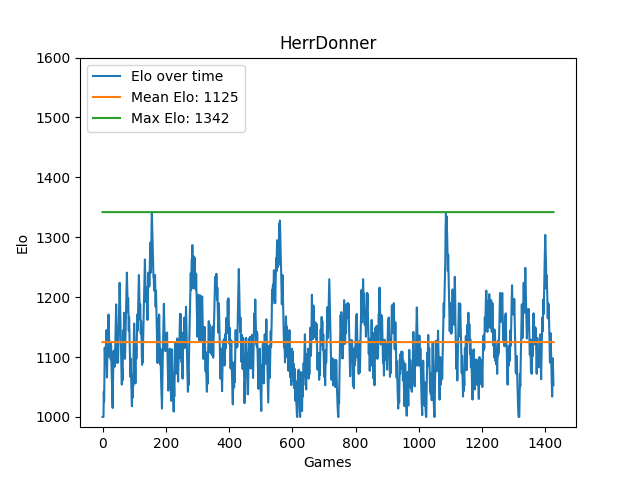
\includegraphics[width=1\linewidth]{images/Donner-Elo-Time.png}
    \captionof{figure}{Elo HerrDonner}
    \label{fig:donner-elo}
  \end{minipage}%
  \begin{minipage}{.5\textwidth}
    \centering
    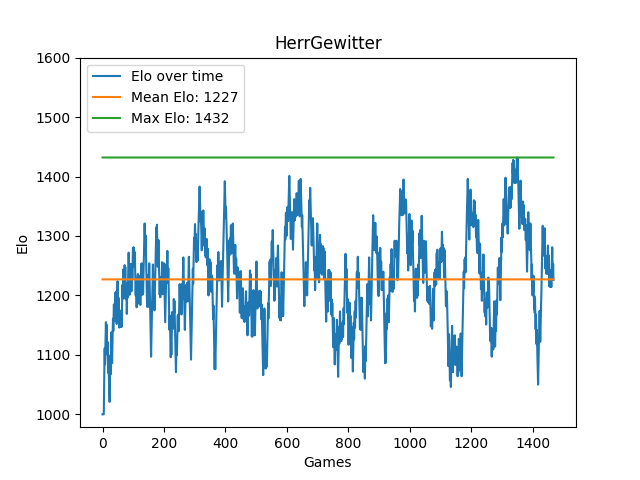
\includegraphics[width=1\linewidth]{images/Gewitter-Elo-Time.png}
    \captionof{figure}{Elo HerrGewitter}
    \label{fig:gewitter-elo}
  \end{minipage}
\end{figure}
\todo{Print this page and check if the figures are to small}
Both agents were evaluated at the same time over the span of multiple days by playing over 1400 ranked games each 
against human opponents on Pokémon Showdown. Figure \ref{fig:donner-elo} shows the Elo rating of \textit{HerrDonner}
over time, while figure \ref{fig:gewitter-elo} displays the Elo rating of \textit{HerrGewitter}. 
\begin{figure}[h]
	\centering
	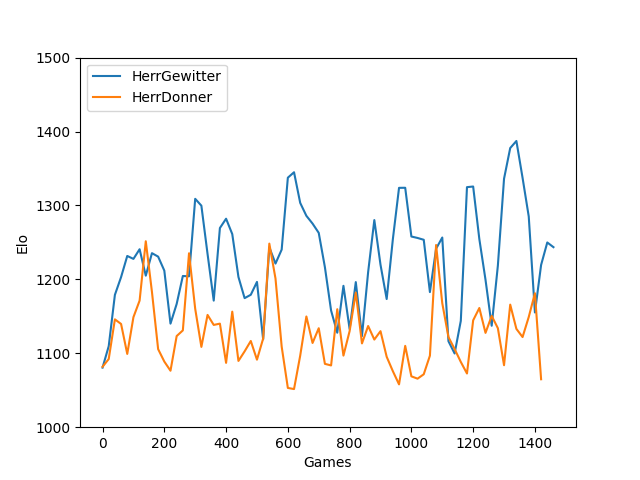
\includegraphics[width=0.7\textwidth]{images/Smoothed-Elo-Time.png}
	\caption{Smoothed Elo}
	\label{fig:elo-smoothed}
\end{figure}
In order to make comparison of both agents more easy, figure \textit{fig:elo-smoothed} shows the smoothed Elo of
both agents over time. Smoothing was achieved by dividing the Elo history in chunks of size 20 and then plotting
the average Elo of each chunk. 
\\\begin{minipage}{\linewidth}
\begin{lstlisting}[language=Python, caption=Smoothing Elo values]
  step = 20
  smoothed_elo = []
  for i in range(0, len(elo_history), step):
      sec = elo_history[i: i + step]
      smoothed_elo += [(i, sum(sec) / len(sec))]
\end{lstlisting}
\end{minipage}
The first thing to note is that \textit{HerrGewitter} has a higher mean Elo ($1227$) as well as a higher max Elo ($1432$)
than \textit{HerrDonner} who achieved an average Elo of $1125$ and peaked at an Elo of $1342$. 
\todo{Why is my agent worse than Pmariglia?}
\begin{table}[h]
  \centering
  \begin{tabular}{|l|c|c|c|c|c|c|}
    \hline
     & Random & MaxDmg & Pmariglia \cite{Github:pmariglia-showdown} & DQN \cite{Huang_Lee_2019} & Donner   & Gewitter  \\
    \hline
    Random                                         & N / A  & -      & -         & 995 / 5   & 992 / 8  & 993 / 7   \\
    \hline
    MaxDmg                                         &        & N / A  & -         & 929 / 71  & 906 / 94 & 951 / 49  \\
    \hline
    Pmariglia                                      &        &        & N / A     & 612 / 388  & -        & 273 / 727 \\
    \hline
    DQN                                            &        &        &           & N / A     & -        & -         \\
    \hline
    Donner                                         &        &        &           &           & N / A    & 580 / 420 \\
    \hline
    Gewitter                                       &        &        &           &           &          & N / A     \\                            
    \hline
    \end{tabular}
    \caption{Battle results of 1,000 games between the agents.}
    \label{tab:agent-performance}
  \end{table}
Table \ref{tab:agent-performance} shows the performance of different agents when directly competing against each other.
\todo{DQN played against an older version of Pmariglia.}
Each entry displays the results of a thousand games played between both agents. The first number indicates the amount
of games the agent in the current column won. There are a multiple things to point out here: \\
While \textit{HerrDonner} and \textit{HerrGewitter} achieved almost similar results when battling a random agent, 
\textit{HerrDonner} performed notably worse against the \textit{MaxDmg} agent which always picks the move with the
highest base power. Also, \textit{HerrDonner} only managed to win $58\%$ against \textit{HerrDonner} despite notably
better results against human players \todo{Above section how hard it is to beat Donner / Gewitter}. 